\documentclass[11pt, a4paper]{article}
\usepackage[nochapters]{classicthesis}                              % template
\usepackage[margin=42mm]{geometry}                                  % margins
\usepackage[utf8]{inputenc}                                         % allow utf-8 input
\usepackage[T1]{fontenc}                                            % use 8-bit T1 fonts
\usepackage{graphicx}                                               % images
\usepackage{url}                                                    % URL typesetting
\usepackage{booktabs}                                               % good-looking tables
\usepackage{multirow}                                               % for tables
\usepackage{amsfonts}                                               % blackboard math symbols
\usepackage{amsmath}                                                % math ops
\usepackage{nicefrac}                                               % compact 1/2, etc.
\usepackage{microtype}                                              % microtypography

\definecolor{darkblue}{rgb}{0, 0, 0.5}                              % define link color
\hypersetup{colorlinks=true,citecolor=darkblue,                     % set link color
            linkcolor=darkblue, urlcolor=darkblue}

% Your packages here
% \usepackage{...}                                                  % some info, maybe

% !!! PLEASE CHANGE THESE VARIABLES TO MATCH YOUR INFORMATION !!!

\def\thesistitle{The Main Title of the Thesis}                      % title
\def\subtitle{The Subtitle of the Thesis If It Has One}             % subtitle
    % ^if there is no subtitle, replace by \def\subtitle{}  
\def\yourname{Stefan Winter}                                                                       % ^first and last name
\def\yourprogramme{Data Science \& Society}                         % OR (remove this)
% \def\yourprogramme{Cognitive Science \& Artificial Intelligence}    % uncomment this
\def\yourstudentnumber{2067606}                                      % ANR (or u-number)
\def\finalmonth{January}
\def\finalyear{2022}
\def\supervisor{Dr. Peter Hendrix}
\def\committee{prof. dr. The Second Reader}
\def\acknowledgments{Some room for acknowledgements.}

% METADATA

\hypersetup{pdfauthor   = \yourname,
            pdftitle    = \thesistitle\ \subtitle,
            pdfsubject  = \yourprogramme\ Master Thesis
}

% CHOOSE EITHER OF -----------------------------------------
% IEEE STYLE:

% \usepackage[square,numbers]{natbib}                               % bracket-style refs
% \usepackage{natbib}                                               % OR: parenthesized refs
% \bibliographystyle{IEEEtranN}

% OR -------------------

\usepackage[natbibapa]{apacite}                                     % only parentheses
\bibliographystyle{apacite}                                         % 'cause APA

% !!! ------------------------------------------------------ !!!

\begin{document}
% DON'T TOUCH THIS FILE, THANKS!

\pagenumbering{gobble}
\thispagestyle{empty}

\newgeometry{margin=30mm}
\begin{center}
\hspace{0.75cm}
\includegraphics[scale=0.5]{logo.eps} \\
\vspace{5cm}
\huge\spacedallcaps{\thesistitle} \\ [0.5cm]
\Large\spacedallcaps{\subtitle} \\ [1.2cm]
\normalsize\spacedallcaps{\yourname{}} \\ [1cm]
\normalsize{\spacedlowsmallcaps{Thesis submitted in partial fulfillment}} \\
\normalsize{\spacedlowsmallcaps{of the requirements for the degree of}} \\
\normalsize{\spacedlowsmallcaps{Master of Science in \yourprogramme{}}}\\
\normalsize{\spacedlowsmallcaps{at the School of Humanities and Digital Sciences}} \\
\normalsize{\spacedlowsmallcaps{of Tilburg University}} \\ [1.5cm]
\end{center}
\restoregeometry

\newpage

\begin{tabular}{l}
\noindent \spacedlowsmallcaps{student number} \\ [0.2cm]
\yourstudentnumber \\ [0.5cm]
\spacedlowsmallcaps{Committee} \\ [0.2cm]
\supervisor \\
\committee\\ [0.5cm]
\spacedlowsmallcaps{location} \\ [0.2cm]
Tilburg University    \\                        
School of Humanities and Digital Sciences \\
Department of Cognitive Science \& \\
Artificial Intelligence \\
Tilburg, The Netherlands \\ [0.5cm]
\spacedlowsmallcaps{date} \\ [0.2cm]
\today \\ \\
\spacedlowsmallcaps{Word Count} \\ [0.2cm]
8700 words
\end{tabular}
\vfill
\begin{tabular}{l}
\spacedlowsmallcaps{acknowledgments} \\ [0.2cm]
\noindent \acknowledgments{} \\ \\
\end{tabular}

\newpage

\newpage \pagenumbering{arabic}

\title{\rmfamily\normalfont\spacedallcaps{\thesistitle}\\[0.2cm]
       \rmfamily\small\spacedallcaps{\subtitle}}
\author{\spacedlowsmallcaps{\yourname}}
\date{}

\maketitle  % don't remove this :)

% --- start writing below:

\begin{abstract}
This is where the abstract goes. Don't forget to change the variables in \texttt{main.tex} to change all general placeholders shown in this document. The \texttt{frontmatter.tex} file should be left alone.
\end{abstract}

\section{Introduction} \label{sec:introduction}

The internet has enabled humankind to access information, exchange ideas and become part of a community. Of course, that also applies to online message boards. Ever since the internet found mainstream adoption, people joined those message boards to discuss trading the stock market. Most recently the Reddit forum wallstreetbets attracted a lot of interest and now counts over 10 million members. In this subreddit, members talk about various investment ideas. However, most of those ideas are of speculative nature with members trying to get rich quick, usually by using risky derivatives like stock options. While the wallstreetbets community undoubtedly minted many millionaires, there are also numerous people who lost their life savings.


Even though the Reddit subforum was already founded in 2012, it got most of its media attention in 2021 due to a short-squeeze of the GameStop (GME) stock that drove the stock price up several hundred percent. However, it was not the rapid price appreciation that amazed market participants. Instead, it was the unprecedented decentralized and coordinated buying of Gamestop shares by members of the wallstreetbets community that attracted attention \citep{anand2021reddit}.
Interestingly, the story repeated itself when forum members sent other stocks, such as AMC Entertainment and BlackBerry to the moon.

Organizing the mass-coordinated buying of stock, however, requires that enough participants share the same sentiment. Some research shows that social media sentiment has a particularly strong impact on uninformed traders 

\begin{quote}
\emph{Can sentiment analysis of the WallStreetBets Reddit-forum be used to predict daily changes in the stock price of Gamestop?}
\end{quote}

\noindent The sub-questions can be listed seperately, as such:

\begin{itemize}
    \item[RQ1] \emph{Which sentiment analysis approach performs best on predefined key performance indicators?}
    \item[RQ2] \emph{How can the domain-specific language of the Reddit forum WallStreetBets best be incorporated into sentiment analysis?}
    \item[RQ3] \emph{Which machine learning algorithm delivers the best predictive performance for changes in daily stock prices of selected securities based on the sentiment analysis performed earlier?}
\end{itemize}

\noindent Or, format it as you desire (tip: you can nest \texttt{itemize} as well). You can alternate \emph{emph} and \textbf{textbf} however you wish. This should cover most of the things required for the introduction.

\section{Related Work}

Copy paste BibTeX code\footnote{Using e.g. the quote icon in GScholar, then BibTeX at the bottom.} and put it in \texttt{references.bib}. After, you can cite some work \citep{mackay2003information} -- using \texttt{\textbackslash citep}. You can refer to the author of e.g. \cite{minsky1961steps} directly like using \texttt{\textbackslash cite} (this does not work when using bracket-citation). If you use bracket-style,\footnote{Find the \texttt{natbib} part in the \texttt{main.tex} \LaTeX{} script.} you might want use \texttt{\textbackslash citeauthor} when citing, like: see \citeauthor{ananny2018seeing} \cite{ananny2018seeing}.  If you want to add pages you can use brackets in \texttt{\textbackslash citep[][p. 5]\{mackay2003information\}}, which looks like: \citep[][p. 5]{mackay2003information}. The first brackets can be used for things like \emph{see}, and \emph{e.g.}. If you want to cite multiple authors, simply comma-separate them (\texttt{\textbackslash citep\{\-minsky\-1961\-steps,\-mackay\-2003\-information\}}) and it will aggregate them automatically \citep{minsky1961steps,mackay2003information}.

\section{Method}

If you define any equations (\verb|\begin{equation}...|), you probably might want to define everything using math operators (e.g., \verb|$D$|) and cite the work (!). So for example, following \cite{lewis1994sequential}, representing a document $d \in D$ as tf$(d)$, we define a probabilistic model $(d | Y = y)$ for all documents in class $y$, and select $y$ most likely to generate $d$:

\begin{equation} \label{eq:nbarg}
    \hat{y} = \underset{y}{\mathrm{argmax}} \ P(d | y) \cdot P(y)
\end{equation}

With this we can detect spam (see Figure~\ref{fig:spam}) or bots.  Note that the figures (and tables for that matter) might not always be placed in this section (oh no)! \LaTeX{} determines where to best put your objects, so don't worry about that. The reader will find them. \textbf{NOTE}: this Figure has a Creative Commons license; you cannot re-use other authors' figures without explicit permission or permissive licensing (as this would mean copyright infringement). You can refer to the equations as well (Equation~\ref{eq:nbarg})!

\begin{figure}
    \centering
    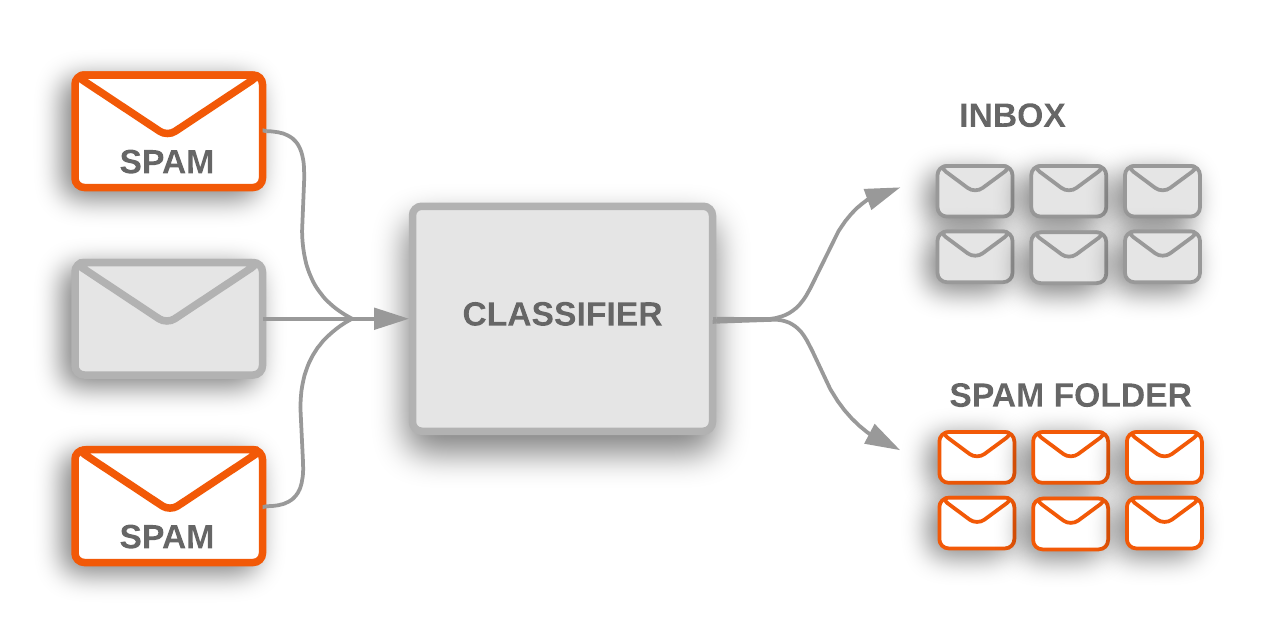
\includegraphics[width=\textwidth]{spam.png}
    \caption{Spam classification example. Source: \href{https://developers.google.com/machine-learning/guides/text-classification}{Google} (CC BY 4.0).}
    \label{fig:spam}
\end{figure}

\section{Results}

\begin{table}
    \caption{Best scoring models classifying bots, on Twitter and Facebook respectively. $F_1$ scores report positive (bot) class. Outline text left (l) and numbers right (r).}
    \label{tab:results}
    \centering
    \small
    \begin{tabular}{llrr}
        \toprule
                              &                                   & \multicolumn{2}{c}{$F_1$ score} \\
                                                                  \cmidrule{3-4}
        PCA                   &  Models                           &  Twitter        &  Facebook       \\ 
        \midrule
        \multirow{3}{*}{300}  & Linear SVM ($C = 0.1$)            &   0.51          & \textbf{0.91} \\
                              & Random Forest ($S = 5, F = 5$)    &   0.71          & 0.85 \\
                              & Naive Bayes                       &   0.61          & 0.73 \\
        \midrule
        \multirow{3}{*}{500}  & Linear SVM ($C = 0.1$)            &   0.55          & 0.84   \\
                              & Random Forest ($S = 5, F = 5$)    &   \textbf{0.76} & 0.71 \\
                              & Naive Bayes                       &   0.41          & 0.64 \\
        \midrule
                              & Majority                          &   0.50          & 0.60 \\
        \bottomrule
    \end{tabular}
\end{table}

You have results and want to show them --- probably in a table of some kind as you can see in Table~\ref{tab:results}. Highlight important scores with \verb|\textbf{}|, use booktabs commands for structure: \verb|\toprule \midrule \bottomrule|. APA does not allow vertical lines.

\subsection{Some Model} \label{subs:model}

If you have anything specific to talk about, use subsections, and refer to them as Section~\ref{subs:model}. Don't use paragraphs or subsubsections.

\section{Discussion}

The results were promising!

\section{Conclusion}

Done.

\bibliography{references}

\section*{Appendix A} \label{app:a}

If you have nothing to append: remove this. You can do a page referral for these, like: Appendix A (page~\pageref{app:a}).

\section*{Appendix B}

And this!
\end{document}